% ============================================================================
\section{Stable Diffusion overview}
% ============================================================================

\begin{frame}[allowframebreaks]{Stable Diffusion}
    \textbf{What is Stable Diffusion?}
    \begin{itemize}
        \item A state-of-the-art text-to-image generative model.
        \item Released by Stability AI and collaborators (2022).
        \item Open-source, enabling wide adoption and customization.
    \end{itemize}
    \begin{figure}
        \centering
        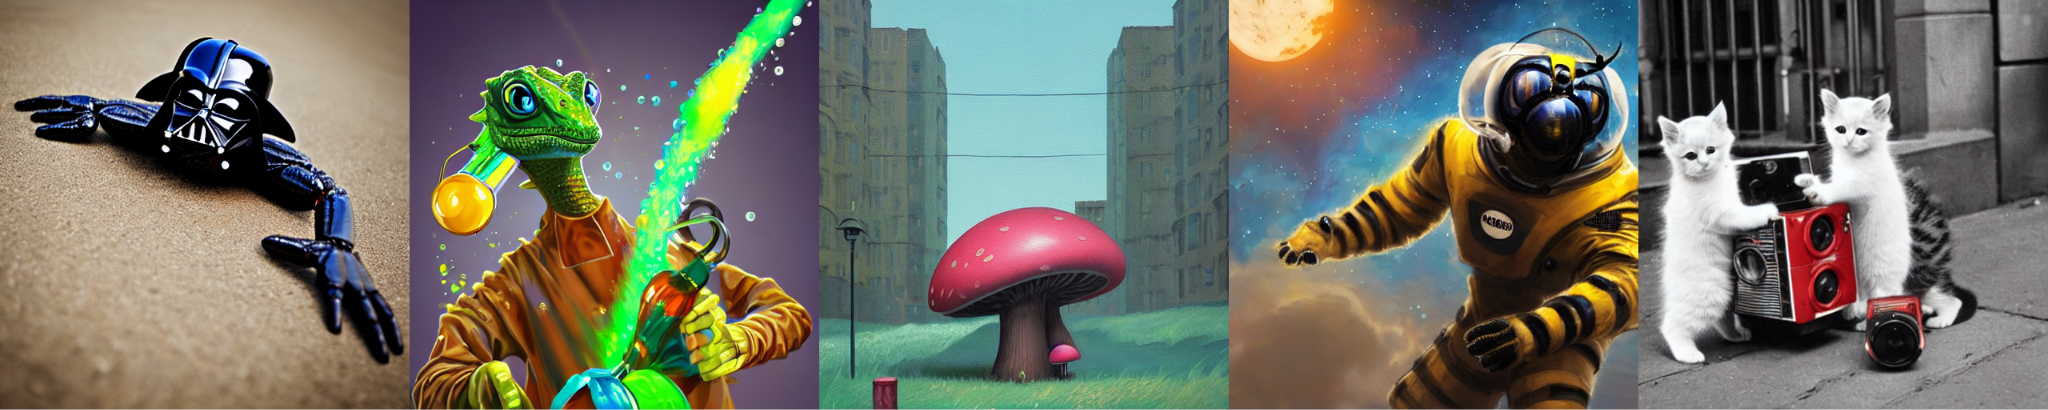
\includegraphics[width=1.06\linewidth,height=\textheight,keepaspectratio]{images/adv-img-gen/slide_99_1_img.png}
    \end{figure}
    
    \framebreak

    \textbf{Advantages}
    \begin{itemize}
        \item High-quality, diverse image generation.
        \item Efficient training and inference due to latent space operations.
        \item Open-source and extensible for research and applications.
    \end{itemize}

    \framebreak

    \textbf{What do we need to make a good generative model?}
    \begin{enumerate}
        \item Method of learning to generate new images \hfill \textbf{Forward/reverse diffusion}
        \item Way to link text and images \hfill \textbf{Text-image representation model}
        \item Way to compress images \hfill \textbf{Autoencoder}
        \item Way to add in good inductive biases \hfill \textbf{U-net architecture} $+$ \textbf{`attention'}
    \end{enumerate}
    \vspace{1em}
    \textit{Making a ‘good’ generative model is about making all these parts work together well!}
\end{frame}






% % --- Frontiers (from sections/diffusion/stable-diffusion-lecture/block4-frontiers.tex) ---
% \begin{frame}{Beyond imagery: applied frontiers}
%   \begin{itemize}
%     \item \textbf{AlphaFold3:} diffusion over 3D molecular coordinates from sequence data.
%     \item \textbf{Diffusion Policy:} action-trajectory generation for robotics from demonstrations.
%     \item \textbf{ControlNet / SDXL:} spatial conditioning and higher-fidelity open models.
%     \item \textbf{Stable Video Diffusion:} temporal layers on top of image LDM backbone.
%   \end{itemize}
%   \vspace{0.5em}
%   Diffusion is now a general-purpose framework for structured generation across modalities.
% \end{frame}
